\documentclass{article}
%% \usepackage{times}
\usepackage[dvipsnames]{xcolor}
\usepackage[table]{xcolor}
\usepackage{latexsym}
\usepackage{url}
\usepackage{hyperref}
\usepackage{lmodern}
\usepackage{graphicx}
\usepackage{mathtools}
\usepackage{amsmath}
\DeclarePairedDelimiter\ceil{\lceil}{\rceil}
\DeclarePairedDelimiter\floor{\lfloor}{\rfloor}
\hypersetup{colorlinks=true}
\graphicspath{ {images/} }
\huge

\usepackage{fancyhdr}
\pagestyle{fancy}
\lhead{CLAUDIA-ELENA CIONTU} % controls the left corner of the header
\chead{} % controls the center of the header
\rhead{\textit{Sisteme Concurente si Distribuite}} % controls the right corner of the header
\lfoot{} % controls the left corner of the footer
\cfoot{} % controls the center of the footer
\rfoot{Page~\thepage} % controls the right corner of the footer
\renewcommand{\headrulewidth}{0.8pt}
\renewcommand{\footrulewidth}{0.8pt}
\begin{document}
\thispagestyle{plain}% Removes the header from the first page. Change plain to empty to remove the numbering entirely.




\begin{center}
\Large
\textcolor{BlueViolet}{{Universitatea din Craiova,\ Facultatea de Automatică, Calculatoare și Electronică}}\\
    \vspace{7mm}
     \end{center} 
    \begin{center}
          
    \textbf{
\includegraphics[scale=0.5]{logo-ace.jpeg}}
\end{center}
% top matter

\title{\textbf{\textit{Atelierul lui Mos Craciun}}}

\vspace{1em}
\LARGE
\textbf{\textcolor{MidnightBlue}{{  Titlu tema}}}: Atelierul lui Mos Craciun

\LARGE
\vspace{1em}
\textbf{\textcolor{MidnightBlue}{{Nume si prenume}}}:Ciontu Claudia-Elena

\LARGE
\vspace{1em}
\textbf{\textcolor{MidnightBlue}{{Grupa}}}: CR3.1 B

\LARGE
\vspace{1em}
\textbf{\textcolor{MidnightBlue}{{Anul de studiu}}}: Anul 3

\LARGE
\vspace{1em}
\textbf{\textcolor{MidnightBlue}{{Specialitatea}}}: Calculatoare si Tehnologia Informatiei



% abstract
\newpage
\renewcommand*\contentsname{\centering \textcolor{blue}{{ Cuprins}}\\
\vspace{1cm} } 
\large \tableofcontents
\newpage
\section{\bfseries\scshape\textcolor{BlueViolet}{Enuntul problemei}}
Craciunul se apropie! Mos Craciun si angajatii sai (elfii si renii) se pregatesc pentru un nou Craciun care aduce bucurie si cadouri tuturor copiilor din jurul lumii.
El este proprietarul unui atelier care contine mai multe fabrici (in fiecare an el reconstruieste fabricile). Angajatii sunt elfii care construiesc jucarii, renii care asteapta sa impacheteze jucariile sub forma de cadouri. Mos Craciun are nevoie disperata ca atelierul sa functioneze, tinand cont ca ultimul manager
batran al atelierului a plecat. Planul atelierului contine reguli care ne asigura ca toate cadourile sunt create la timp astfel incat nici un copil sa nu ramana fara darul de Craciun. Mos Craciun doreste sa-l ajuti la implementarea planului fabricii utilizand concurenta in Java.


\subsection{\textcolor{Periwinkle}{Lucruri necesare}}
Fluxul de control concurent in acest exemplu este destul de subtil. Miscarea elfilor (ce include si raportarea la fabrica) este initiata independent de fiecare elf, fiecare ruland pe cate un fir separat. \\
\\
Astfel ca elfi diferiti se pot misca si raporta la fabrica in mod concurent. Raportarea concurenta la fabrica trebuie realizata in mod sincronizat.
Apelul de raportare declanseaza metoda individuala de raportare pentru toti elfii inregistrati la fabrica.\\
\\
Acest aspect trebuie tratat cu grija deoarece ambele metode de raportare si miscare sunt sincronizate, astfel ca nu vor putea fi apelate concurent pentru un acelasi obiect.
\subsection{\textcolor{Periwinkle}{Indicatii}}
Mos Craciun stie ca il puteti ajuta. El stie ca aveti la dispozitie urmatoarele instrumente utile de programare concurenta:\\
--- Semafoare, monitoare si zavoare\\
--- Fire de executie. Fiecare elf poate fi reprezentat de un fir separate de executie in cadrul planului atelierului\\
--- Ele trebuie sa comunice: elfii creaza cadouri si renii le primesc pentru a le transmite lui Mos Craciun care le va livra copiilor\\
--- Mos Craciun vrea ca renii sa-I transmita cadourile prin TCP/IP, pentru a nu se pierde nici un cadou.\\

\section{\textcolor{BlueViolet}{Schita Aplicației.}}\label{sec_tr}
\subsection{\textcolor{CadetBlue}{Ansamblul arhitectural al aplicatiei}}
  \begin{center}
    \textbf{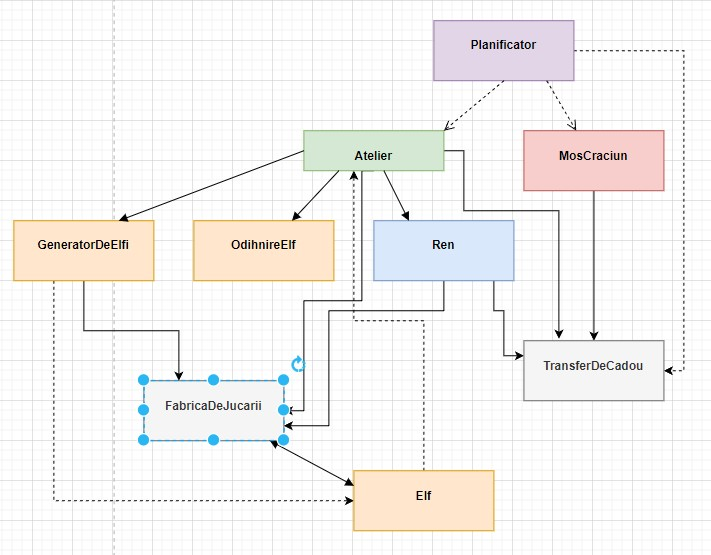
\includegraphics[scale=1.0]{Arhitectura.jpg}}
\end{center}
\subsubsection{\textcolor{Periwinkle}{Planificator.java}}
\textcolor{Mulberry}{Planificator} este  punctul de plecare al aplicației 

In Planificator  :
\begin{itemize}
\item \textcolor{Orchid}{Cadou} - v-a creea coada de transfer de cadouri
\item \textcolor{Orchid}{MosCraciun} - il vom creeaza pe Moș Crăciun
\item \textcolor{Orchid}{atelier} - creează atelierul lui Moș Crăciun
\item \textcolor{Orchid}{atelier.creazaFabrici()}- începe să creeze fabrici
\item \textcolor{Orchid}{MosCraciun.start()} - Si Moș Crăciun începe să primească cadouri de la Reni
\end{itemize}

\subsubsection{\textcolor{Periwinkle}{MosCraciun.java}}
\textcolor{BrickRed}{MosCraciun} este  o clasa ce implementează un fir care se va comporta ca Moș Crăciun.


 
\begin{itemize}
\item \textcolor{Bittersweet}{Cadou} - creeaza o coada de transfer de cadouri
\item  \textcolor{Bittersweet}{Run}  - il va creea pe Moș Crăciun
\end{itemize}


\subsubsection{\textcolor{Periwinkle}{Atelier.java}}
\textcolor{ForestGreen}{Atelier} este clasa unde se creeaza atelierul lui Moș Crăciun

In Atelier avem :
\begin{itemize}
\item  \textcolor{LimeGreen}{nrFabrici} - numărul de fabrici existente
\item \textcolor{LimeGreen}{fabrici} - toate fabricile existente
\item \textcolor{LimeGreen}{generatoare} - toate firele de elf generati existenti
\item \textcolor{LimeGreen}{nrElfi} - numărul total de elfi existenți
\item \textcolor{LimeGreen}{elfiCounterLock} - un lacăt pentru numărul de elfi existenti
\item \textcolor{LimeGreen}{reni} - toți renii existenți
\item \textcolor{LimeGreen}{cadou} - mijloc de transfer de cadouri între Moș Crăciun și reni
\item \textcolor{LimeGreen}{elfPensionareSemaphore} - un semafor pentru pensionarea elfilor
\item \textcolor{LimeGreen}{elfPensionare} - un subiect pentru pensionarea elfilor
\item \textcolor{LimeGreen}{getElfiCounterLock} - returnează blocarea contorului elfilor
\item \textcolor{LimeGreen}{creazaFabrici} - creează toate fabricile, generatorii de elfi, renii și începe executarea lor
\end{itemize}


\subsubsection{\textcolor{Periwinkle}{Ren.java}}
\textcolor{Cyan}{Ren} este clasa unde vom implementa un fir ce se comportă ca un ren

In Ren :
\begin{itemize}
\item  \textcolor{CornflowerBlue}{Numar}- numărul/numele renului (identificare)
\item \textcolor{CornflowerBlue}{fabrici} - toate fabricile existente
\item \textcolor{CornflowerBlue}{Cadou} - mijlocul de transfer al cadourilor
\item \textcolor{CornflowerBlue}{run} - thread-ul va executa următoarele acțiuni:\\
--- primește un cadou de la o fabrică\\
--- dă cadoul lui Moș Crăciun prin Cadou\\
--- doarme între 10-30 de milisecunde
\item \textcolor{CornflowerBlue}{giveCadouLuiMosCraciun} - oferă un cadou Moșului
\item \textcolor{CornflowerBlue}{extrageCadouDinFabrica} - intră într-o fabrică aleatorie dintre cele existente și ia un cadou de acolo
\end{itemize}


\subsubsection{\textcolor{Periwinkle}{OdihnireElf.java}}
\textcolor{YellowOrange}{OdihnireElf} este clasa unde vom implementa un thread folosit pentru a retrage un elf aleatoriu

In OdihnireElf :
\begin{itemize}
\item \textcolor{Dandelion}{run} - thread-ul  va executa următoarele acțiuni într-o buclă:\\
--- elibereaza un permis al semaforului de pensionare pentru ca un elf sa se poata retrage\\
--- doarme 50 de milisecunde

\end{itemize}

\subsubsection{\textcolor{Periwinkle}{GeneratorDeElfi.java}}
\textcolor{YellowOrange}{GeneratorDeElfi} este clasa unde vom implementa un fir ce se comportă ca un ren

In GeneratorDeElfi :
\begin{itemize}
\item  \textcolor{Dandelion}{fabrica}- fabrica pentru care thread-ul va genera elfi
\item \textcolor{Dandelion}{run} - thread-ul va executa următoarele acțiuni:\\
--- genereaza un elf \\
--- doarme între 500-1000 de milisecunde
\item \textcolor{Dandelion}{generareElf} - thread-ul va executa următoarele acțiuni:\\
---creează un nou elf dacă este posibil (Avem conditia ca numărul de elfi existenți în fabrică sa fie mai mic decât jumatate din dimensiunea fabricii)\\
---adaugă elful în fabrică și crește numărul total de elfi

\end{itemize}


\subsubsection{\textcolor{Periwinkle}{FabricaDeJucarii.java}}
\textcolor{CadetBlue}{FabricaDeJucarii} este clasa unde se creeaza atelierul lui Moș Crăciun

In Atelier avem :
\begin{itemize}
\item  \textcolor{Gray}{numar} - numarul fabricii
\item \textcolor{Gray}{N} - dimensiunea fabricii matriceala
\item \textcolor{Gray}{elfi} -elfi din fabrica
\item \textcolor{Gray}{cadouri} -cadourile din fabrica
\item \textcolor{Gray}{fabricaLock} - un lacat pentru accesarea matricei din fabrică
\item \textcolor{Gray}{listaElfiLock} -un lacat pentru accesarea elfilor din fabrică 
\item \textcolor{Gray}{reniSemaphore} - un semafor pentru maximul de elfi permisi dn lista
\item \textcolor{Gray}{cadouriLock} - un lacat pentru accesarea cadourilor din lista 
\item \textcolor{Gray}{getFabricaLock} - returnează lacatul matricei din fabrică
\item \textcolor{Gray}{nrExistentiDeElfi} - returneaza numarul existenti de elfi din fabrica
\item  \textcolor{Gray}{getN} - returneaza dimensiunea matriceala a fabricii
\item \textcolor{Gray}{getNumar} - returneaza numarul fabricii
\item \textcolor{Gray}{run} - thread-ul v-a executa:\\
---v-a "intreba"(ask)toti elfii positia actuala\\
---dormi pentru 3000milisecunde
\item \textcolor{Gray}{mutaElf} -v-a muta un elf in fabrica astfel:\\
---obtine toate informatiile despre elf(pozitie,nr cadouri si numarul elfului)\\
---incearca sa se mute intr- directie daca poate insa daca e inconjurat,se opreste .
\item \textcolor{Gray}{mutareSpreStanga} -verifica daca elful se poate muta spre stanga
\item \textcolor{Gray}{mutareSpreDreapta} - verifica daca elful se poate muta spre sdreapta
\item \textcolor{Gray}{mutareInJos} - verifica daca elful se poate muta in jos
\item \textcolor{Gray}{mutareInSus} - verifica daca elful se poate muta in sus
\item \textcolor{Gray}{adaugaElf} - adauga un nou elf creat in fabrica
\item \textcolor{Gray}{askPositiaElfilor} - intreaba elfii despre pozitia actuala
\item \textcolor{Gray}{getCadou} - reni obtin cadourile de la fabrica
\item \textcolor{Gray}{creeazaCadou} -creeaza cadourile(le adauga in lista de cadouri)
\item \textcolor{Gray}{pensionareElf} -pensioneaza(retrage)un elf din fabrica
\end{itemize}

\subsubsection{\textcolor{Periwinkle}{TransferDeCadou.java}}
\textcolor{CadetBlue}{TransferDeCadou} este clasa unde se creeaza atelierul lui Moș Crăciun

In TransferDeCadou avem :
\begin{itemize}
\item  \textcolor{Gray}{head} - primul din lista(capul)
\item \textcolor{Gray}{tail} - ultimul din lista(coada)
\item \textcolor{Gray}{cadouri} - numarul de cadouri ce trebuie transferate
\item \textcolor{Gray}{receiveGift} -asa reuseste Mos Craciun sa primeasca cadourile de la reni
\item \textcolor{Gray}{giveCadou} - asa reusesc reni sa ii dea lui Mos Craciun cadourile
\end{itemize}

\subsubsection{\textcolor{Periwinkle}{Elf.java}}
\textcolor{YellowOrange}{Elf} implementeaza un thread care sa se comporte ca un elf

In Elf :
\begin{itemize}
\item  \textcolor{Dandelion}{Numar}-Numarul elfului(se v-a comporta ca si un nume)
\item \textcolor{Dandelion}{X} - coordonata pe axa X a elfului in fabrica matriceala
\item \textcolor{Dandelion}{Y} - coordonata pe axa Y a elfului in fabrica matriceala
\item  \textcolor{Dandelion}{cadou}-cadoul actual pe care l-a creat elful
\item \textcolor{Dandelion}{fabrica} - fabrica ce contine elful actual
\item \textcolor{Dandelion}{run} - elful v- executa :\\
---creeaza un cadou nou\\
---isi schimba pozitia prin fabrica\\
---se odihneste(sleep) pentru 30 milisecunde\\
---incearca sa se pensioneze
\item  \textcolor{Dandelion}{stopWork}-opreste elful pentru 10-50 milisecunde
\item \textcolor{Dandelion}{raporteazaPozitia} - raporteaza positia actuala a elfului in fabrica matriceala
\item \textcolor{Dandelion}{schimbaPozitia} - incerca sa isi schimbe pozitia (mai precis coordonatele) 
\item  \textcolor{Dandelion}{getNumar}-returneaza numarul(numele) elfului nostru
\item \textcolor{Dandelion}{getX} - returneaza coordonatele pe axa X a elfului in fabrica matriceala
\item \textcolor{Dandelion}{getY} - returneaza coordonatele pe axa Y a elfului in fabrica matriceala
\item \textcolor{Dandelion}{getCadou} - returneaza cadoul actual al elfului
\end{itemize}

\section{\bfseries\scshape\textcolor{BlueViolet}{Sarcini suplimentare}}
\subsection{\textcolor{CadetBlue}{Retragerea unui Elf}}
A fost creat un nou thread pentru retragerea unui elf, care eliberează un permis de retragere la fiecare 50 de milisecunde. Fiecare elf se va muta în fabrică și apoi va încerca să obțină un permis de plecare. Când un elf se retrage din fabrică, acesta este șters din matricea fabricii, precum și din lista de spiriduși existenți.
\subsection{\textcolor{CadetBlue}{“Odihnirea” unui elf}}
\subsubsection{\textcolor{Periwinkle}{Semaphores}}
Când un elf atinge diagonala principală, acesta va încerca să obțină un semafor pentru a schimba contorul pentru elfii care așteaptă la barieră, apoi asteapta până când contorul este mai mic de N. 
\subsubsection{\textcolor{Periwinkle}{CyclicBarrier}}
Când un elf ajunge pe diagonala principală, acesta va rămâne la barieră până când toți N elfi vor trece prin ea, apoi își va relua operațiunile obișnuite (mutare în fabrică).

\section{\bfseries\scshape\textcolor{BlueViolet}{Rezultate obtinute}}
\subsection{\textcolor{CadetBlue}{Atelierul Lui Mos Craciun}}
\begin{center}
    \textbf{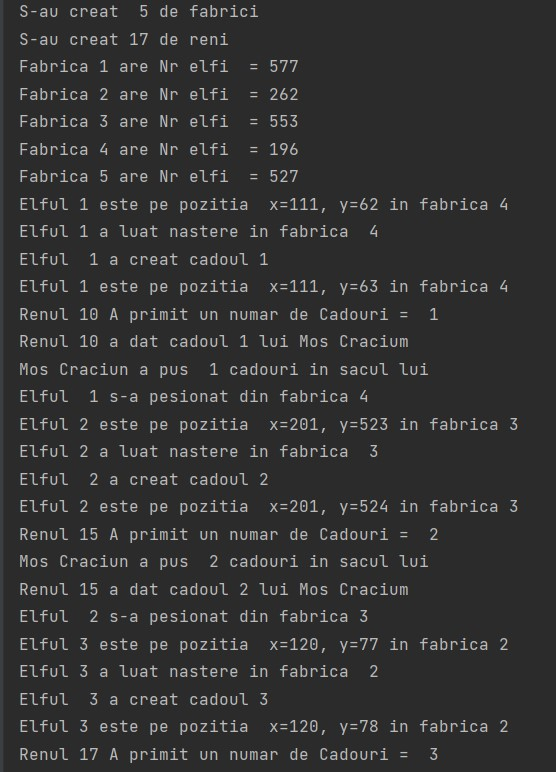
\includegraphics[scale=0.8]{1.jpg}}
\end{center}\\
Un semafor cu 10 permisiuni pentru fiecare fabrică (maximum 10 reni pot ajunge în fabrică în același timp) a fost folosit pentru a sincroniza intrările în fabrică de reni. Permisele au fost obținute atunci când un ren a primit un cadou de la fabrica.\\

Deoarece am vrut să atribui fiecărui elf un număr unic care să-i identifice la nivel global și nu în fiecare fabrică, am folosit un lacăt pentru a împiedica doi elfi să aibă același număr.\\

Am folosit o pentru a transmite cadouri de la reni către Moș Crăciun, sincronizând procedurile de adăugare a unui cadou la coadă și ștergerea unui cadou din coadă.\\
\subsection{\textcolor{CadetBlue}{Atelierul Lui Mos Craciun-Semaphores}}
\begin{center}
    \textbf{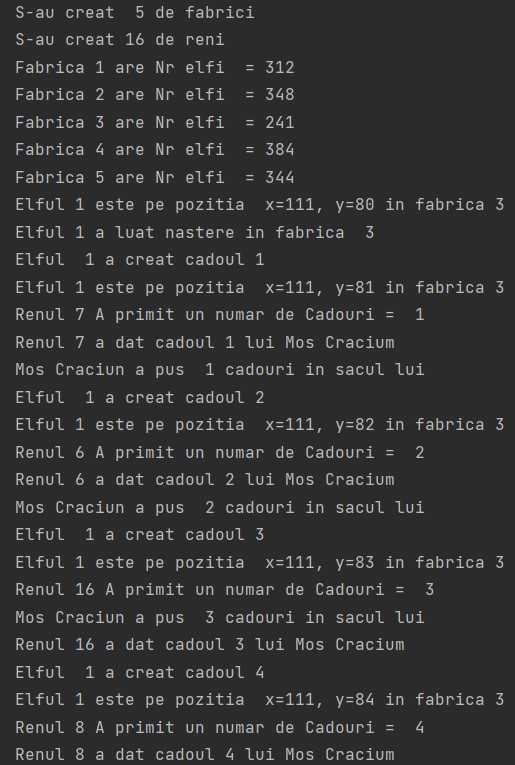
\includegraphics[scale=0.8]{2.jpg}}
\end{center}
\subsection{\textcolor{CadetBlue}{Atelierul Lui Mos Craciun-CyclicBarrier}}
\begin{center}
    \textbf{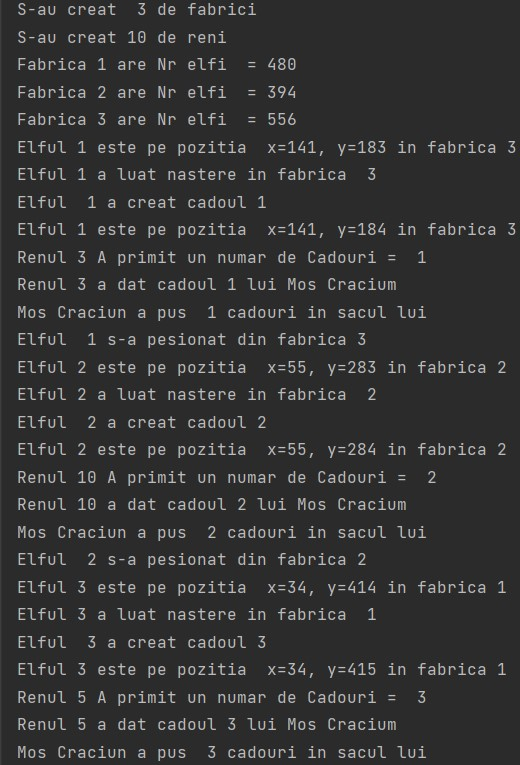
\includegraphics[scale=0.8]{3.jpg}}
\end{center}
\section{\textcolor{BlueViolet}{Referinte}}\label{sec_ed}
\url{https://www.overleaf.com/project}\\\\
\url{https://www.geeksforgeeks.org/semaphore-in-java/}\\\\
\url{https://www.geeksforgeeks.org/importance-of-thread-synchronization-in-java/}\\\\
\url{https://docs.oracle.com/javase/7/docs/api/java/util/concurrent/Semaphore.html}\\\\
\url{https://docs.oracle.com/javase/7/docs/api/java/util/concurrent/CyclicBarrier.html}\\\\
\url{https://docs.oracle.com/javase/7/docs/api/java/util/concurrent/locks/ReentrantLock.html}\\\\
\url{https://www.jetbrains.com/idea/download/?fromIDE=#section=windows}\\\\
\end{document}
